\tikzsetnextfilename{two_flavor_ensemble_threshold_anotated}%
\begin{tikzpicture}
    \node[above right, inner sep=0] (image) at (0,0) {
        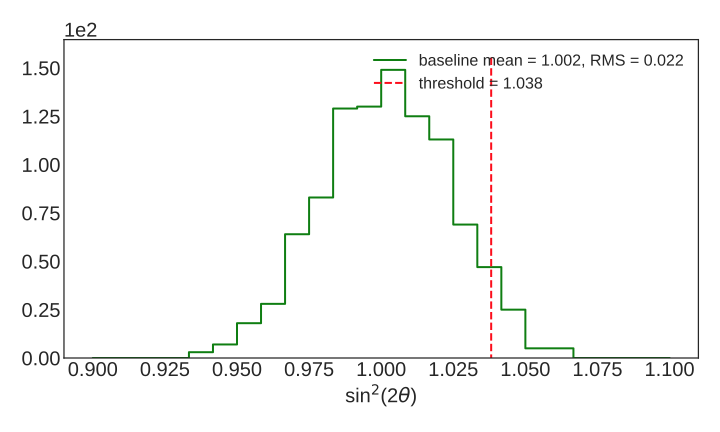
\includegraphics[width=0.8\linewidth]{figures/measurement/three_flavor/ensemble_pre_fit/two_flav_ensemble_threshold.png}
    };
    % Create scope where axes are the plot coordinates
    \begin{scope}[
        x={($0.4*(image.south east)$)},
        y={($0.45*(image.north west)$)},
        shift={($0.13*(image.south east) + 0.17*(image.north west)$)}
    ]
        % Grid
        %\draw[darkgray,step=.25] (0,0) grid (2,1.5);
        % x-coordinates start at 0.9 and one unit = 0.1
        \draw (1.23, 0) -- node [sloped, font=\footnotesize, anchor=south] {observed $=1.023$} (1.23, 1.3);
    \end{scope}
\end{tikzpicture}